\chapter{Aufgabe}

Die Aufgabe bestand in einer Implementierung eines Webservices in PHP mit dem Slim Framework.
Als Zusatzaufgabe sollte das Thema WS-Security durch Authentifizierung mittels OAuth2 und Verschlüsselung mittels HTTPS gelöst werden.

Der Webservice stellt die Vermietungsplattform für einen fiktiven Bikesharingdienst dar.

\chapter{Installation}
\section{Datenbank}
Für die Installation der Datenbank müssen die mitgelieferten Dumps bikesharingservice.sql und bikesharingservice\_oauth.sql in eine MySQL Datenbank eingefügt werden.
\begin{lstlisting}[caption={Datenbankimport}\label{lst:dbimport},captionpos=b] 
mysql -u root -p -h localhost
mysql> create database bikesharingservice;
mysql> create database bikesharingservice_oauth;
mysql> exit;
mysql -u username -p -h localhost bikesharingservice < bikesharingservice.sql
mysql -u username -p -h localhost bikesharingservice_oauth < 
	bikesharingservice_oauth.sql
\end{lstlisting}
Anschließend muss die Datenbank gestartet werden.

\section{Webservice und API}

\chapter{Funktionen Webservice}

\begin{tabularx}{\columnwidth}{|X|p{1.5cm}|X|p{1.5cm}|}
	\hline
	Name & Method & URL & Access \\
	\hline
	\hline
	Alle verfügbare Fahrradstationen & GET & /stations & public \\
	\hline
	Spezielle Station & GET & /stations/stationID & public \\
	\hline
	Alle verfügbaren Fahrräder & GET & /bikes & public \\
	\hline
	Spezielles Fahrrad & GET & /bikes/bikesID & public \\
	\hline
	Alle Fahrradmodelle & GET & /models & public \\
	\hline
	Spezielles Fahrradmodell & GET & /models/modelID & public \\
	\hline
	Alle Buchungen & GET & /bookings & protected \\
	\hline
	Buchung erstellen & POST & /bookings & protected \\
	\hline
	Einzelne Buchung & GET & /bookings/bookingID & protected \\
	\hline
	Einzelne Buchung stornieren & DELETE & /bookings/bookingID & protected \\
	\hline
	Einzelne Buchung bearbeiten & PUT & /bookings/bookingID & protected \\
	\hline
	Accountinformationen & GET & /account & protected \\
	\hline
\end{tabularx}

\section{GET Methoden}
\subsection{stations}
Liefert eine Liste aller verfügbaren Stationen zurück an denen Fahrräder
zum Verleih zur Verfügung stehen.

\begin{longtable}[c]{@{}lll@{}}
\toprule\addlinespace
Method & URL & Access
\\\addlinespace
\midrule\endhead
GET & /stations & public
\\\addlinespace
\bottomrule
\end{longtable}

\subsubsection{Parameter}\label{parameter}

\begin{longtable}[c]{@{}lll@{}}
\toprule\addlinespace
Name & Required & Description
\\\addlinespace
\midrule\endhead
location & nein & Standort an dem nach Stationen gesucht werden soll,
z.B. ``Dresden'' oder ``Berlin''
\\\addlinespace
model & nein & ID eines bestimmten Fahrradmodells nach dem gefiltert
werden soll, z.B. 105 oder 185
\\\addlinespace
\bottomrule
\end{longtable}

\subsubsection{Request Example}\label{request-example}

\begin{verbatim}
GET /stations?location=Dresden&model=105
\end{verbatim}

\subsubsection{Response}\label{response}

Liefert eine Liste von verfügbaren Stationen zurück, jede Station
besteht aus den folgenden Parametern: * stationId - Die einzigartige
Kennung der Station * name - Der Name der Station * longitude -
Längengrad * latitude - Breitengrad * bikes - Die Anzahl an zum Verleih
zur Verfügung stehenden Fahrräder in der Station * description - Die
ausführliche Beschreibung der Station * pictureUrl - Die URL eines Fotos
von der Station

\subsubsection{Response Examples}\label{response-examples}

\begin{verbatim}
{
   "stations" : [
      {
         "stationId" : 64,
         "name" : "Hauptbahnhof",
         "longitude" : -33.8670522,
         "latitude" : 151.1957362,
         "bikes" : 78,
         "description" : "Tolle Station am Hauptbahnhof, direkt vor dem Ausgang.",
         "pictureUrl" : "www.test.de/station64.jpg"
      },
      {
         "stationId" : 82,
         "name" : "Zoo",
         "longitude" : -33.8670522,
         "latitude" : 151.1957362,
         "bikes" : 108,
         "description" : "Eine Station direkt am Zoo.",
         "pictureUrl" : "www.test.de/station82.jpg"
      }
   ]
}
\end{verbatim}

\subsection{bikes}
Liefert eine Liste aller verfügbaren Fahrräder die zum Verleih zur
Verfügung stehen.

\begin{longtable}[c]{@{}lll@{}}
\toprule\addlinespace
Method & URL & Access
\\\addlinespace
\midrule\endhead
GET & /bikes & public
\\\addlinespace
\bottomrule
\end{longtable}

\subsubsection{Parameter}\label{parameter}

\begin{longtable}[c]{@{}lll@{}}
\toprule\addlinespace
Name & Required & Description
\\\addlinespace
\midrule\endhead
location & ja & Standort an dem nach verfügbaren Fahrrädern gesucht
werden soll, z.B. ``Dresden'' oder ``Berlin''
\\\addlinespace
radius & nein & Radius in dem um die location gesucht werden soll in
Meter (default: 2500), z.B. 5000
\\\addlinespace
modelId & nein & Die eindeutige Kennung eines bestimmten Fahrradmodells
nach dem gefiltert werden soll, z.B. 105 oder 185
\\\addlinespace
stationId & nein & Die eindeutige Kennung einer bestimmten
Verleihstation nach der gefiltert werden soll, z.B. 46 oder 4
\\\addlinespace
\bottomrule
\end{longtable}

\subsubsection{Request Example}\label{request-example}

\begin{verbatim}
GET /bikes?location=Dresden&radius=5000&modelId=105&stationId=4
\end{verbatim}

\subsubsection{Response}\label{response}

Liefert eine Liste von verfügbaren Fahrrädern, jedes Fahrrad besteht aus
den folgenden Parametern: * bikeId - Die einzigartige Kennung des
Fahrrads * modelId - Die einzigartige Kennung des Fahrradmodells * price
- Der Preis für 15 Minuten in Cent. * longitude - Längengrad * latitude
- Breitengrad * stationId - Falls das Fahrrad in einer Verleihstation
steht, ist dies die eindeutige Kennung der Station * distance - Die
Entfernung zum gewählten Standort

\subsubsection{Response Examples}\label{response-examples}

\begin{verbatim}
{
   "bikes" : [
      {
         "bikeId" : 46,
         "modelId" : 105,
         "price" : 100,
         "longitude" : -33.8670522,
         "latitude" : 151.1957362,
         "stationId" : 4,
         "distance": 2800
      },
      {
         "bikeId" : 34,
         "modelId" : 105,
         "price" : 150,
         "longitude" : -33.8670522,
         "latitude" : 151.1957362,
         "stationId" : 4 ,
         "distance": 2800
      }
   ]
}
\end{verbatim}

\subsection{models}
Liefert eine Liste aller verfügbaren Fahrradmodelle.

\begin{longtable}[c]{@{}lll@{}}
\toprule\addlinespace
Method & URL & Access
\\\addlinespace
\midrule\endhead
GET & /models & public
\\\addlinespace
\bottomrule
\end{longtable}

\subsubsection{Parameter}\label{parameter}

\begin{longtable}[c]{@{}lll@{}}
\toprule\addlinespace
Name & Required & Description
\\\addlinespace
\midrule\endhead
location & nein & Standort an dem nach verfügbaren Fahrrädern gesucht
werden soll, z.B. ``Dresden'' oder ``Berlin''
\\\addlinespace
stationId & nein & Die eindeutige Kennung einer bestimmten
Verleihstation nach der gefiltert werden soll, z.B. 46 oder 4
\\\addlinespace
\bottomrule
\end{longtable}

\subsubsection{Request Example}\label{request-example}

\begin{verbatim}
GET /models?location=Dresden&stationId=4
\end{verbatim}

\subsubsection{Response}\label{response}

Liefert eine Liste von verfügbaren Fahrradmodellen, jedes Modell besteht
aus den folgenden Parametern: * modelId - Die einzigartige Kennung des
Fahrradmodells * name - Der Name des Fahrradmodells * description - Eine
Beschreibung des Modells * pictureUrl - Die URL eines Fotos, welches das
Fahrradmodell zeigt * bikes - Die Anzahl an zum Verleih zur Verfügung
stehenden Fahrräder dieses Modells

\subsubsection{Response Examples}\label{response-examples}

\begin{verbatim}
{
   "models" : [
      {
         "modelId" : 105,
         "name" : "Rennrad",
         "description" : "Bestens geeignet für das Fahren auf dem Asphalt.",
         "pictureUrl" : "www.test.de/model105",
         "bikes" : 78
      },
      {
         "modelId" : 68,
         "name" : "Kinderfahrrad",
         "description" : "Geeignet für Kinder zwischen 6 und 9 Jahren.",
         "pictureUrl" : "www.test.de/model68",
         "bikes" : 8
      }
   ]
}
\end{verbatim}

\subsection{account}
Liefert die Accountinformationen des Nutzers.

\begin{longtable}[c]{@{}lll@{}}
\toprule\addlinespace
Method & URL & Access
\\\addlinespace
\midrule\endhead
GET & /account & protected
\\\addlinespace
\bottomrule
\end{longtable}

\subsubsection{Request Example}\label{request-example}

\begin{verbatim}
GET /account
\end{verbatim}

\subsubsection{Response}\label{response}

Liefert die Accountinformationen des Nutzers, ein Account besteht aus
den folgenden Parametern: * accountId - Die einzigartige Kennung des
Nutzers * email - Die E-Mail Adresse des Nutzers

\subsubsection{Response Examples}\label{response-examples}

\begin{verbatim}
{
   "accountId" : 1696,
   "email" : "test@test.com"
}
\end{verbatim}

\subsection{bookings}
Liefert eine Liste aller getätigten Buchungen.

\begin{longtable}[c]{@{}lll@{}}
\toprule\addlinespace
Method & URL & Access
\\\addlinespace
\midrule\endhead
GET & /bookings & protected
\\\addlinespace
\bottomrule
\end{longtable}

\subsubsection{Request Example}\label{request-example}

\begin{verbatim}
GET /bookings
\end{verbatim}

\subsubsection{Response}\label{response}

Liefert eine Liste aller getätigten Buchungen, jede Buchung besteht aus
den folgenden Parametern: * bookingId - Die einzigartige Kennung der
Buchung * bikeId - Die einzigartige Kennung des gebuchten Fahrrads *
date - Das Datum der Buchung

\subsubsection{Response Examples}\label{response-examples}

\begin{verbatim}
{
   "bookings" : [
      {
         "bookingId" : 1682,
         "bikeId" : 105,
         "date" : "2013-12-01 18:44:36"
      },
      {
         "bookingId" : 1696,
         "bikeId" : 168,
         "date" : "2013-12-01 18:45:24"
      }
   ]
}
\end{verbatim}

\section{POST Methoden}
\subsection{bookings}
Erstellt eine einzelne Buchung.

\begin{longtable}[c]{@{}lll@{}}
\toprule\addlinespace
Method & URL & Access
\\\addlinespace
\midrule\endhead
POST & /bookings & protected
\\\addlinespace
\bottomrule
\end{longtable}

\subsubsection{Request Example}\label{request-example}

\begin{verbatim}
POST /bookings
Params: {
   "id": 168
}
\end{verbatim}

\subsubsection{Parameter}\label{parameter}

\begin{longtable}[c]{@{}lll@{}}
\toprule\addlinespace
Name & Required & Description
\\\addlinespace
\midrule\endhead
id & ja & Die einzigartige Kennung des Fahrrads, z.B. 168
\\\addlinespace
\bottomrule
\end{longtable}

\subsubsection{Response}\label{response}

Liefert eine einzelne getätigte Buchung, die Buchung besteht aus den
folgenden Parametern: - 
\begin{itemize}
\item id - Die einzigartige Kennung der Buchung
\item bikeId - Die einzigartige Kennung des gebuchten Fahrrads
\item date - Der Zeitpunkt der Buchung
\end{itemize}

\subsubsection{Response Examples}\label{response-examples}

\begin{verbatim}
{
   	"bookingId" : 1696,
   	"bikeId" : 168,
   	"date" : "2013-12-01 18:45:24"
}
\end{verbatim}

\section{DELETE Methoden}
\subsection{bookings}
Storniert eine einzelne Buchung.

\begin{longtable}[c]{@{}lll@{}}
\toprule\addlinespace
Method & URL & Access
\\\addlinespace
\midrule\endhead
DELETE & /bookings/bookingId & protected
\\\addlinespace
\bottomrule
\end{longtable}

\subsubsection{Request Example}\label{request-example}

\begin{verbatim}
DELETE /bookings/1696
\end{verbatim}

\section{PUT Methoden}
\subsection{bookings}
Ändert eine einzelne Buchung.

WICHTIG: Content-Type: application/x-www-form-urlencoded

\begin{longtable}[c]{@{}lll@{}}
\toprule\addlinespace
Method & URL & Access
\\\addlinespace
\midrule\endhead
PUT & /bookings/bookingId & protected
\\\addlinespace
\bottomrule
\end{longtable}

\subsubsection{Request Example}\label{request-example}

\begin{verbatim}
PUT /bookings/bookingId
Params: {
   "bikeId": 168
}
\end{verbatim}

\subsubsection{Parameter}\label{parameter}

\begin{longtable}[c]{@{}lll@{}}
\toprule\addlinespace
Name & Required & Description
\\\addlinespace
\midrule\endhead
bikeId & nein & Die einzigartige Kennung des Fahrrads, z.B. 168
\\\addlinespace
\bottomrule
\end{longtable}

\subsubsection{Response}\label{response}

Liefert die geänderte Buchung, die Buchung besteht aus den folgenden
Parametern: - bookingId - Die einzigartige Kennung der Buchung - bikeId
- Die einzigartige Kennung des gebuchten Fahrrads - date - Der Zeitpunkt
an dem die Buchung getätigt wurde

\subsubsection{Response Examples}\label{response-examples}

\begin{verbatim}
{
   "bookingId" : 1696,
   "bikeId" : 168,
   "date" : "2013-12-01 18:45:24"
}
\end{verbatim}


\chapter{Webclient}

Der Webclient ist so konzipiert, dass prinzipiell auch mobile Endgeräte unterstützt werden.
Er bietet alle Funktionen die im vorhergehenden Kapitel beschrieben sind.
Dazu zählen eine Suche, sowohl nach Adressen, als auch nach Ausleihstationen, eine Übersicht über die verfügbaren Fahrradmodelle und über die Stationen an denen Fahrräder ausgeliehen werden können.

\begin{figure}[h]
        \centering
	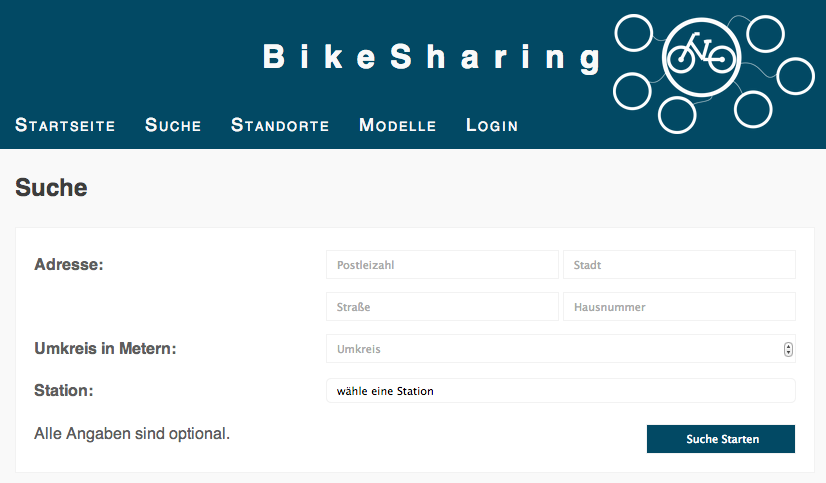
\includegraphics[height=80mm]{pics/bikesharing_search.png}
\end{figure}

\chapter{Zusatzaufgabe WS-Security}

\section{OAuth2}

Das Architekturkonzept von OAuth2 wird durch folgendes Schema verdeutlicht.

\begin{figure}[h]
        \centering
	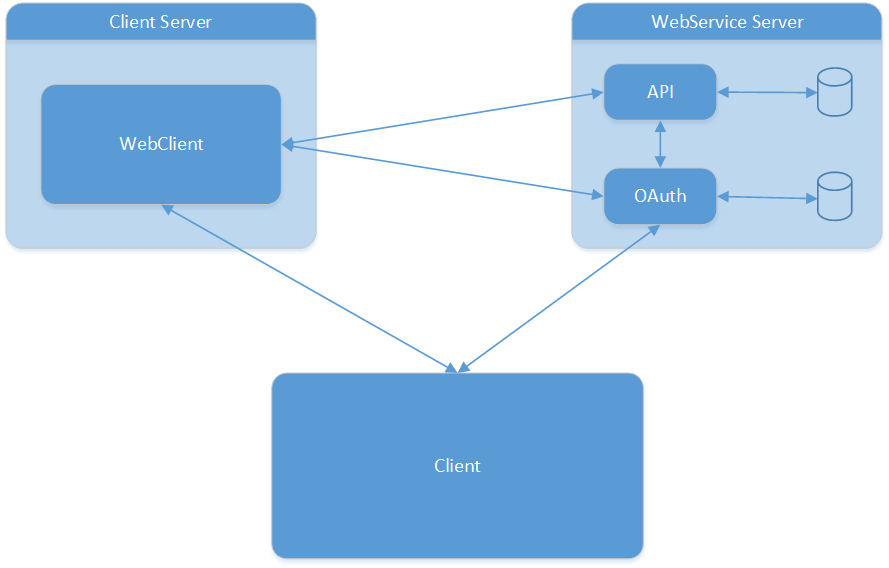
\includegraphics[height=80mm]{pics/Architektur.png}
\end{figure}

\section{Implementierung}

\chapter{Fazit}

Die Implementierung des Webclient ist nach Vorlage einer durchdachten API gut machbar.

Das Slim-Framework war eine gute Wahl, da die Verwendung sehr einfach und fehlerfrei verlief.
Die OAuth-Middleware hat leider nicht funktioniert, auch ist die Implementierung eines OAuth-Servers relativ kompliziert.

Der Aufwand ist, ja nach gewählter Aufgabe, recht hoch, insbesondere wenn man, wie in diesem Fall, Programmiersprachen wählt, die den Teammitgliedern gar nicht, oder nur rudimentär geläufig sind.
Wir hatten uns ursprünglich für PHP entschieden, da wir eine neue Programmiersprache kennenlernen wollten.

%\chapter{Quellen}

